\documentclass[letterpaper,twoside,12pt,french]{report}
\usepackage[utf8]{inputenc}
\usepackage[T1]{fontenc}
\usepackage{babel}
\usepackage[top=2.5cm,bottom=2.5cm,left=2.5cm,right=2.5cm,asymmetric]{geometry}
\usepackage{hyperref}
\usepackage{hypcap}
\usepackage{titlesec}
\usepackage{ragged2e}
\usepackage{hyphenat}
\usepackage{berasans}
\usepackage{setspace}
\usepackage{natbib}
\usepackage{float}

\usepackage{abstract}
\renewcommand{\abstractname}{}
\renewcommand{\absnamepos}{empty}
\renewcommand*\familydefault{\sfdefault}
\usepackage[T1]{fontenc}

\usepackage{graphicx}
\graphicspath{{diagrams/}}

\hypersetup{pdftex,colorlinks=true,allcolors=blue}
\newcommand{\reportTitle}{\uppercase{Détection de modèle humain\\Pour application de réalité augumentée}}
\newcommand{\reportAuthors}{Vincent \uppercase{Boiteau-Robert\\BOIV14029409}\\Marc-Antoine \uppercase{Hébert\\HEBM14019401}\\Julien \uppercase{Lemonde\\LEMJ20059208}\\Alexandre \uppercase{Malo\\MALA0702940}}

\newcommand{\abbrItem}[2]{\item[\uppercase{\textbf{#1}} -] #2}
\setlength{\parskip}{1cm plus4mm minus3mm}

\titleformat
{\chapter}
[display]
{\bfseries\Large}
{}
{0ex}
{
    \vspace{0.2ex}
}
{
    \vspace{-0.5ex}
}

\titleformat
{\section}
[display]
{\bfseries\normalsize}
{}
{0ex}
{
    \vspace{-0.5ex}
}
{
    \vspace{-0.5ex}
}

\begin{document}
\setlength{\parindent}{0cm}\setlength{\parskip}{2ex minus 0.2ex}
\pagenumbering{Roman}
\begin{titlepage}
    \begin{center}
        \uppercase{Rapport technique de projet de fin d'études\\Présenté à l'école de technologie supérieure\\Dans le cadre du cours GTI795 Projet de fin d'études en TI}
        \vfill
        \textbf{\reportTitle}
        \vfill
        \reportAuthors
        \vfill
        \uppercase{Département de génie logiciel et TI}
        \vfill
        \textbf{Professeur-superviseur\\Carlos Vazquez}
        \vfill
        \uppercase{Montréal, 25 avril 2018\\Hiver 2018\\Université du Québec}
    \end{center}
\end{titlepage}
\cleardoublepage
\begin{abstract}
    \begin{center}
        \textbf{\uppercase{\Large{Résumé}}}
        \vspace{2ex}
        \\ \textbf{\reportTitle}
        \\ \vspace{1\baselineskip}
        \reportAuthors
        \\ \vspace{1\baselineskip}
        text résumé ici
    \end{center}
    \vspace{-\baselineskip}
\end{abstract}
\tableofcontents
\listoftables
\listoffigures
\chapter*{\uppercase{Liste des abbréviations}}
\begin{enumerate}
        \abbrItem{ÉTS}{École de Technologie Supérieure}
\end{enumerate}
\cleardoublepage
\pagenumbering{arabic}
\chapter*{\uppercase{Introduction}}
\addcontentsline{toc}{chapter}{INTRODUCTION}
La perforamnce des caméras des appareils mobiles est en constance croissance depuis quelques
années. Ce qui permet d'envisager l'usage de ces appareils dans des nouveaux domaines d'activités.
Un de ces domaine est la réalité augmentée, où la superposition d'éléments virtuels sur une
capture de l'environnement réel en temps réel. Une démocratisation du développement d'application
utilisant cette technologie c'est fait au cours de l'année précédente, 2017. En effet, la nouvelle
interface de programmation applicative ARKit conçu par appel offre un environnement de
développement simplifié au développur d'applications \citep*{StattN2017}. Toutefois, ces technologies
permettent l'interaction avec des modèles généré de façon synthétique. Un défi qui n'a pas encore
de solution reconnue est l'usage de modèles provenant de l'environnement de l'utilisateur dans la
réalité augmentée. Certaines technologies offrent des pistes de solution, mais leur taux d'adoption
et le nivewu de compatibilité avec les autres outils de l'environnement de développement Apple sont
limités.
\par
Une des technologies les plus intéressante est le Structure Sensor\citep*{molitchHou01}. Celle-ci
consiste en un périphérique qui doit être attacher à l'appareil. Le périphérique ajoute une caméra
et un senseur 3D. Avec l'usage de la caméra de l'appareil, celui de l'appareil ont peut avoir une
meilleur compréhension de l'environnemetn 3D. L'outils vient avec une trousse de développement
logiciel permettant de prendre les coordonées d'un objets sous quatres dimensions, x, y, z et la
couleur. Toutefois cette solution n'est pas très connu et a un nombre de ressources limités.
\par
Les deux technologies décrites plus haut apporte chacune des possibilités très intéressantes pour
le développement d'application de réalité augmentée. L'usa\hyp{}ge des fonctionnalité d'une dans l'autre
serait très intéressante. Toutefois au moment où l'équipe a débuté le projet, il n'y a pas
d'interface une telle combinaison. Les deux interfaces utilisent la caméra, par contre chacun
utilise un utilitaire différent pour le contrôle de celle-ci. Les deux utilisent des modèles
numériques 3D, mais chacun a choisi une norme différente. En effet, le Structure Sensor permet
l'extraction en Modèle I/O. Alors que le ARKit utilise les modèles de type scène qui est un format
propriètaire à Apple. Le principal défi du projet consistera à la combinaison de plusieurs
interfaces de programmation pour créer un outils fonctionnel.
\par
Comme décrit dans la section précédente, le principal objectif du projet est la création d'une
interface entre deux technologies mobiles, soit un périphérique d'acquisition de modèle 3D, le
Structure Sensor et la trousse de développement de réalité augmentée d'Apple. Autrement dit,
l'équipe s'attend en fin de session d'avoir produit une application mobile permettant la prise
de modèle à l'aide du senseur. L'application permettra d'ajouter un modèle extrait sur une surface
plane. L'application permet cette chaîne d'action avec une expérience utilisateur agréable et
naturelle à l'utilisateur.
\par
L'application décrite ci-haut représente les attentes pessimistes par rapport aux résultats finaux.
Toutefois, une telle application apporte un éventail de possibilités sur la manipulation de
l'environnement augmentée. Par exemple, une des retombées envisageables et
commercialisable est la numérisation de catalogue de magasin comme Ikea. L'usager peut
donc ajouter un item dans une pièce de sa maison. Si plusieurs couleurs sont disponibles pour
un modèle, chacune des variantes seront disponibles à la modélisation.
\par
Une autre ouverture technologique, qu'une telle application apporterait, est dans un contexte
d'animation 3D. En effet, la création d'un modèle permettrait l'ajout d'un squelette dans celui-ci.
Une fois le squelette créé l'animation du modèle pourrait être fait. Cette possibilité est
particulièrement intéressante pour l'équipe en charge du projet. Dans l'éventualité où la vision
de base du projet sera complétée avant la fin de la session d'Hiver 2018, l'équipe compte se
concentrer sur la création de ce squelette et possiblement la manipulation de celui-ci. La création
de positionnement clé des noueds du squelette pourra être enregistrer afin de permettre l'animation.
L'animation libre est un trop grand défi étant donné les contraintes de temps.
\par
L'objectif principal semble réaliste pour l'équipe de développement étant donné les interfaces déjà
présente pour chacune des technologies. Toutefois, le défi reste important étant donné le manque de
cohérence entre les différentes technologies. Le manque de documentation et de support pour le
Structure Sensor risque d'amener un ensemble de défi supplémentaire.
\par
Par contre, l'équipe de développement considère le temps disponible à la résolution d'un tel enjeu
adéquat. L'expérience en recherche d'information et apprentissage autonome acquis au cours des
formations et stages des membres de l'équipe laisse envisager un succès
\par
Pour ce qui est en la complétion des objectifs accessoire, les limitations de temps rendent
l'estimation de succès plus difficile. Par contre, il est clair que la réalisation de ceux est
apporterait un plus considérable à l'expérience de chacun des membres. La motivation de l'équipe
face à l'enjeu améliore les propabilité de terminer ces objectifs.
\par
Ce rapport consite donc en un suivi des étapes qui permettront de valider ou invalider les
hypothèses décrite si haut. Afin de résoudre un tel défi, l'équipe a du se fier sur les
documentations disponibles en lien avec les technologies ciblés. Un résumé de celles qui ont été
utiles à la résolution du problème sera présenté.
\par
Par la suite, une présentation de la méthodologie utilisée par l'équipe sera décrite. Les étapes
ayant permis la conception de la solution seront par la suite présentées. Une analyse sur le produit
obtenue sera explorer. Afin de clore le projet, les possibilité que la solution apporte à un groupe voulant poursuivre ou
implémenter un projet semblables seront expliquées. L'équipe fera s'est recommandation en fonction
de l'expérience acquise lors du développement.
\chapter*{\uppercase{Revue de la documentation}}
\addcontentsline{toc}{chapter}{REVUE DE LA DOCUMENTATION}
Afin de réaliser le projet, l'équipe de développement a du faire des recherche préliminaire. Les
technologies utilisées n'étaient pas maitrisées par l'équipe au démarrage du projet. Donc, les
recueille de documentation et les projets exemples présents sur internet ont été une bonne source
d'information.
\par
Cette section présentera donc ces ressources pour les grandes parties du projets,
soit le périphérique Structure Sensor, la trousse de développement logiciel de réalité augmentée de
Apple et la gestion de projet.
\section*{Structure Sensor}
\addcontentsline{toc}{section}{Structure Sensor}
Occipital, la compagnie propriétaire du périphérique, publie régulièrement une version de leur
trousse de développement logiciel exposant des interfaces de programmation. La dernière version
publier par la compagnie est la version 0.7.1 en février 2018. \citep*{occipitalsdk} La version du
SDK étant inférieur à 1.0.0, on comoprends que la première version complète est encore en
développement.
\par
Dans l'état actuel, le SDK fourni quand même une liste d'interface disponible dans deux fichiers,
Structure et StructureSLAM. Le permier est composé des différentes interfaces de contrôle du
périphérique. Alors que le deuxièeme est un regroupement des classes permettant le contrôle des
mailles en position tridimensionnelles et les textures de ceux-ci.
\par
Ces interfaces seront la base de la conception du module de prise de modèle grâce au périphérique.
Les tâches de chacunes des interfaces ont été identifiées lors de la lecture du code des entêtes
des interfaces en Objective-C. L'équipe a produit un diagramme de classe afin d'améliorer la
compréhension des responsabilité de chacune des interfaces et les relations entre celles-ci,
Celui-ci est présenté à la page suivante.

\begin{figure}[H]
    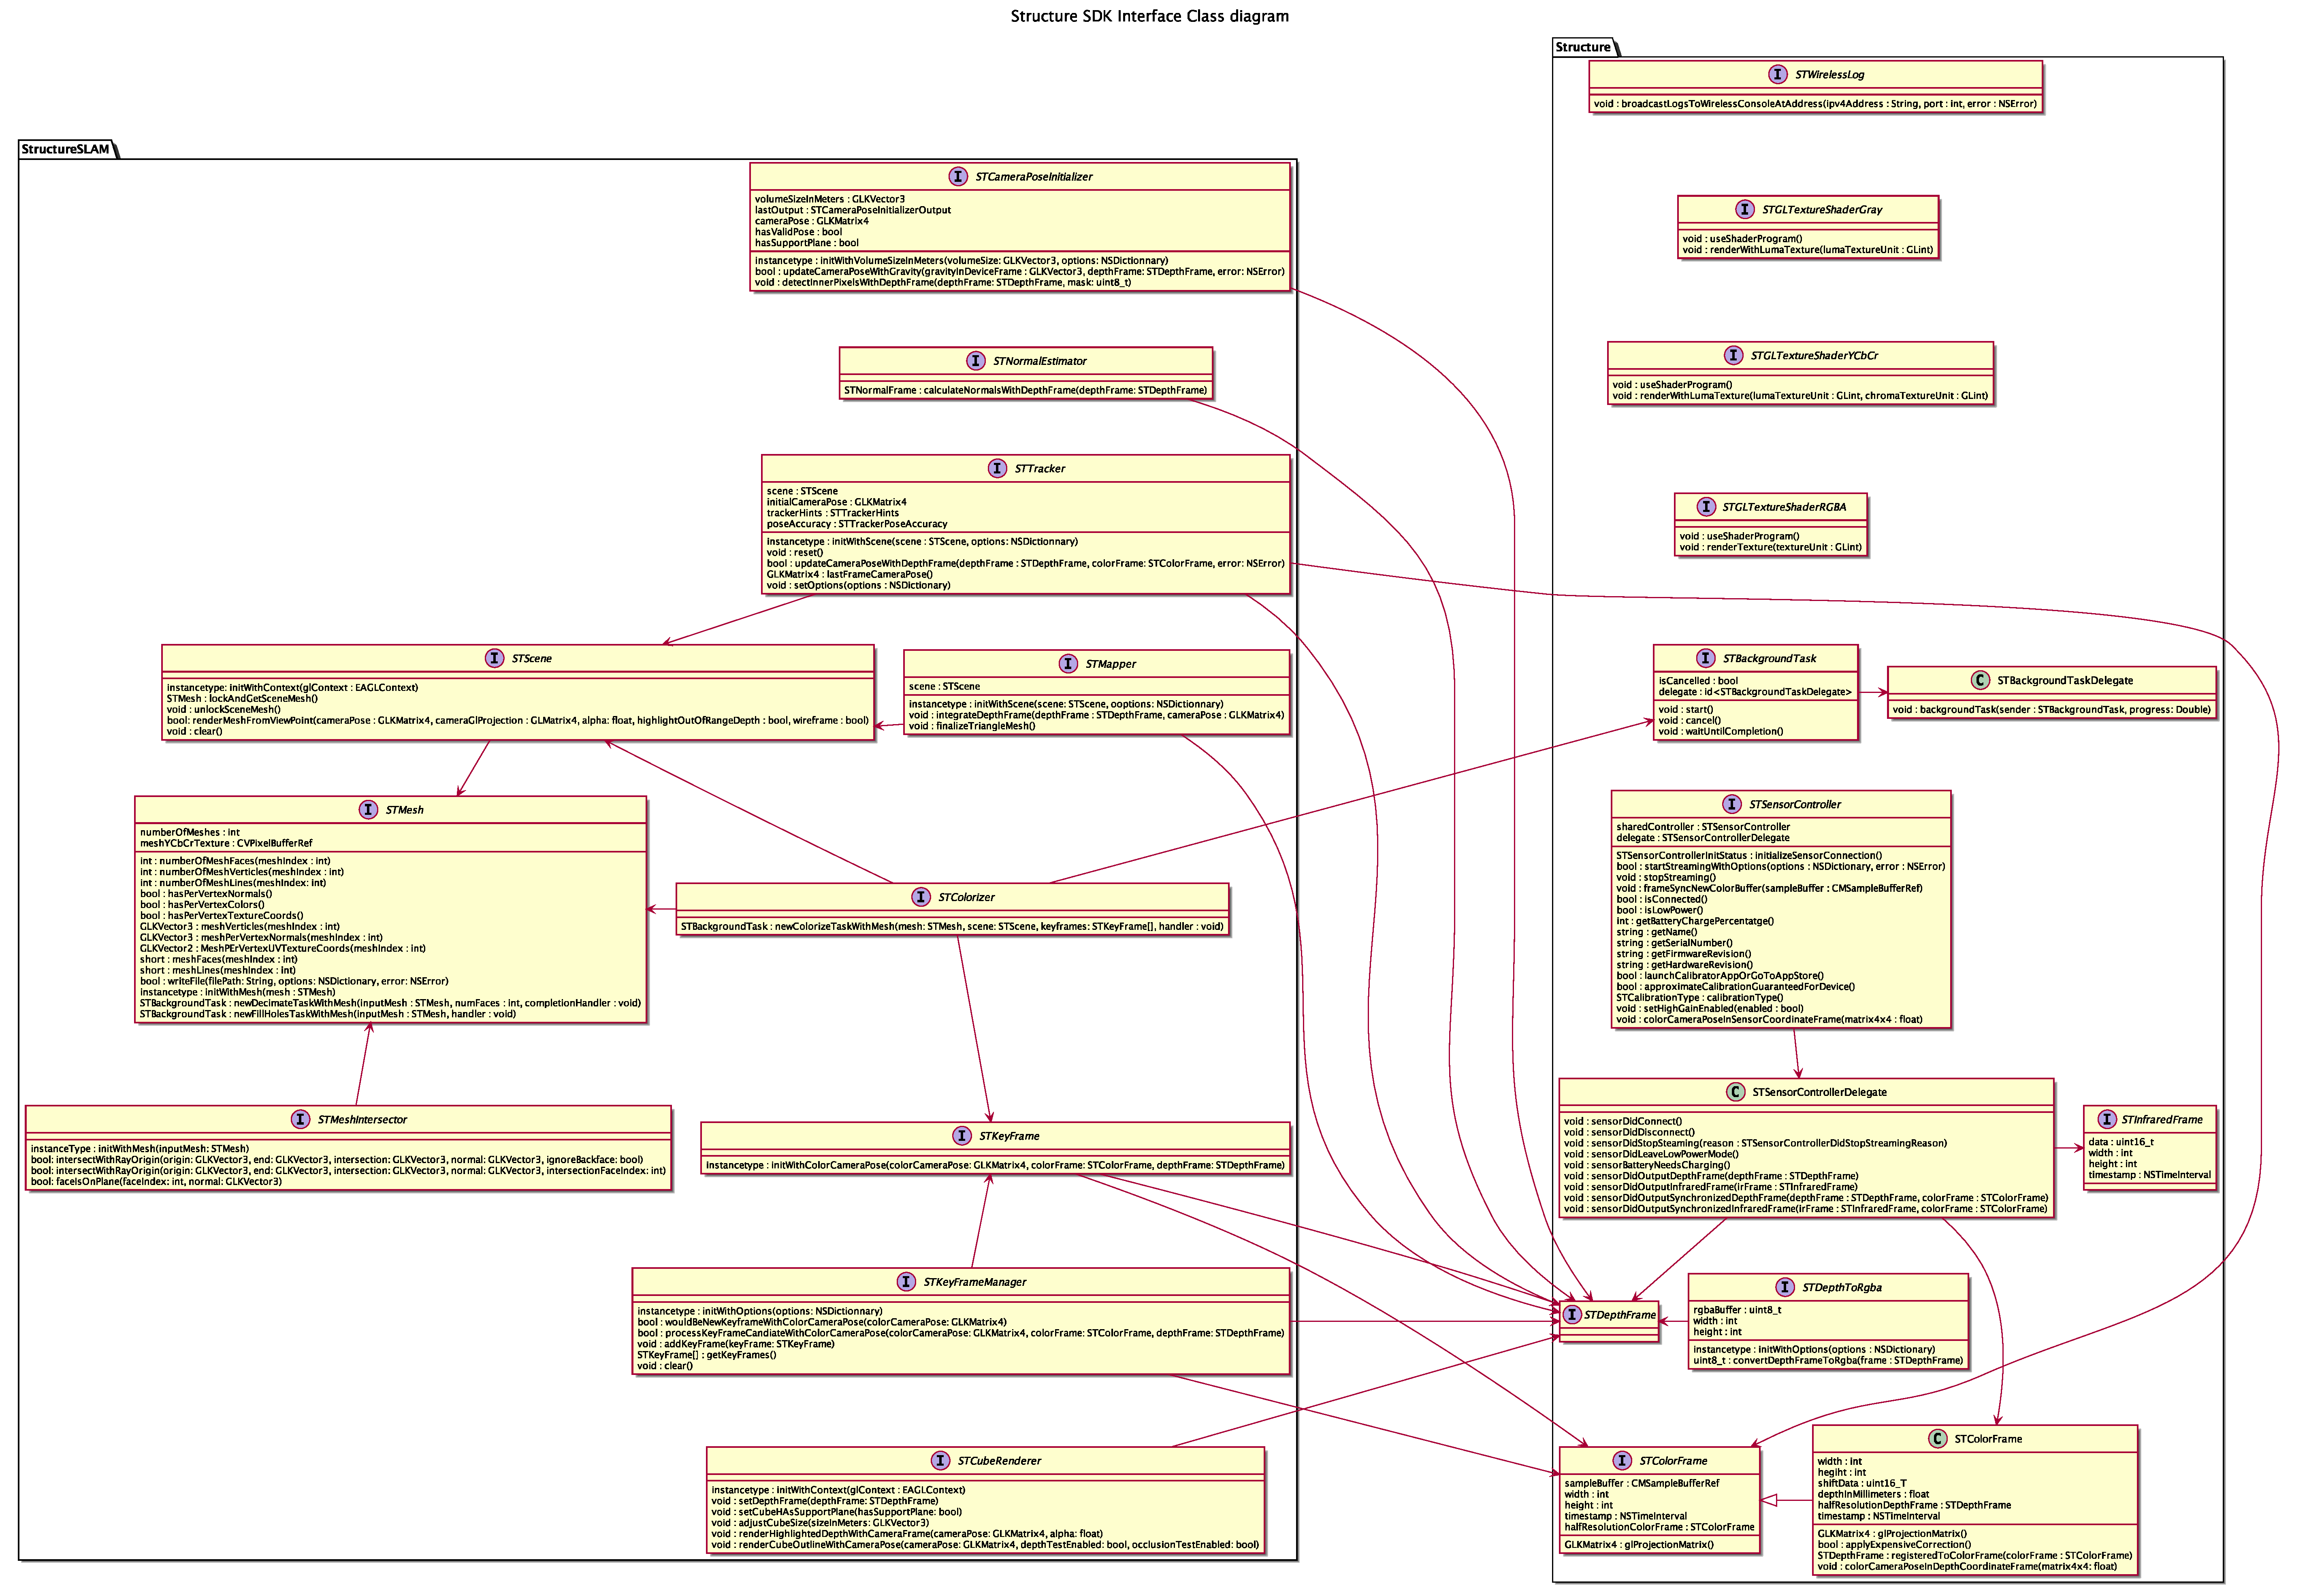
\includegraphics[width=\textwidth]{StructureClassDiagram.eps}
\centering
    \caption{Diagramme de classes du Structure Sensor SDK}
\end{figure}

Dans le diagramme, on constate que plusieurs patrons de conception ont été utilisé et exposé dans
l'interface. La classe STSensorControllerDelegate servira de point d'ancrage entre notre
applications et le Structure Sensor. Cette interface permet donc de réduire les communication ou 
les recherches d'informations dans la logique d'affaire. La plus part de l'usage du SDK dans
l'application devra être fait par cette classe. \citep*{bpse01}
\par
Le Structure Sensor utilise les DepthFrame et ColorFrame pour comprendre l'environnement dans lequel
il est utilisé. Ces concepts ont été introduits par Kinect un des premiers Senseurs 3D ayant connu
un succès commercial étant donné sont intégration dans l'environnement Xbox 360 de Microsoft.
\citep*{microsoft01}
\par
Le Structure SDK contient aussi plusieurs exemples d'application afin de guider les développeurs dans
le développement de leurs applications. Le plus intéressant pour l'objectif du projet est le
Scanneur. Celui-ci permet de convertir un objet dans l'espace de test en un modèle 3D et l'envoyer
par courriel. D'autre fonction inclus dans cet exemple sont la colorisation du modèle et les
différentes options de capture. L'espace de capture est aussi indiqué par un cube et un plan
utilisant les couleurs pour indiquer les objets qui peuvent être capturer.
\chapter*{\uppercase{Méthodologie de travail}}
\addcontentsline{toc}{chapter}{MÉTHODOLOGIE DE TRAVAIL}
méthodologie text
\chapter*{\uppercase{Processus de conception}}
\addcontentsline{toc}{chapter}{PROCESSUS DE CONCEPTION}
processus text
\chapter*{\uppercase{Discussion}}
\addcontentsline{toc}{chapter}{DISCUSSION}
discussion text
\chapter*{\uppercase{Conclusion}}
\addcontentsline{toc}{chapter}{CONCLUSION}
conclusion text
\newpage
\begin{spacing}{1}
    \nocite{*}
    \bibliographystyle{bibETS}
    \addcontentsline{toc}{chapter}{BIBLIOGRAPHIE}

    \bibliography{biblio_fr}
\end{spacing}
\end{document}
